\documentclass[simplex.tex]{subfiles}
% NO NEED TO INPUT PREAMBLES HERE
% packages are inherited from simplex.tex; you can compile this on its own

\onlyinsubfile{
\title{NeuroData SIMPLEX Report: Subfile}
}

\begin{document}
\onlyinsubfile{
\maketitle
\thispagestyle{empty}

The following report documents the progress made by the labs of Randal~Burns and Joshua~T.~Vogelstein at Johns Hopkins University towards goals set by the DARPA SIMPLEX grant.

%%%% Table of Contents
\tableofcontents

%%%% Publications
\bibliographystyle{IEEEtran}
\begin{spacing}{0.5}
\section*{Publications, Presentations, and Talks}
\vspace{-20pt}
\nocite{*}
{\footnotesize	\bibliography{simplex}}
\end{spacing}
%%%% End Publications
}


\subsection{ndreg}

The Large Deformation Diffeomorphic Metric Mapping (LDDMM) algorithm is
an image registration method used to compute a smooth invertible
transform $\phi_{10}$ which aligns template image $I_0$ to target
image $I_1$. The log Jacobian determinant of the mapping $\log
|D\phi_{10}|$ measures local volume change during LDDMM.  Wherever it’s
negative the template CLARITY brain expanded to match the targeted Allen
Reference Atlas (ARA).  Wherever it’s positive the CLARITY brain
contracted.  Figure~\ref{fig:ndreg} shows the $\log |D\phi_{10}|$ overlaid
on a CLARITY brain and a histogram of its values.  It’s clear that this
brain expanded in most places to match the ARA.  This was also the case
for 8 of 9 of the of the other brains.  Our calculations showed that
CLARITY brains were 21\% smaller than the ARA on average.  This likely
occurred due to shrinkage introduced by the CLARIfying processing.


\begin{figure}[h!]
\begin{cframed}
\centering
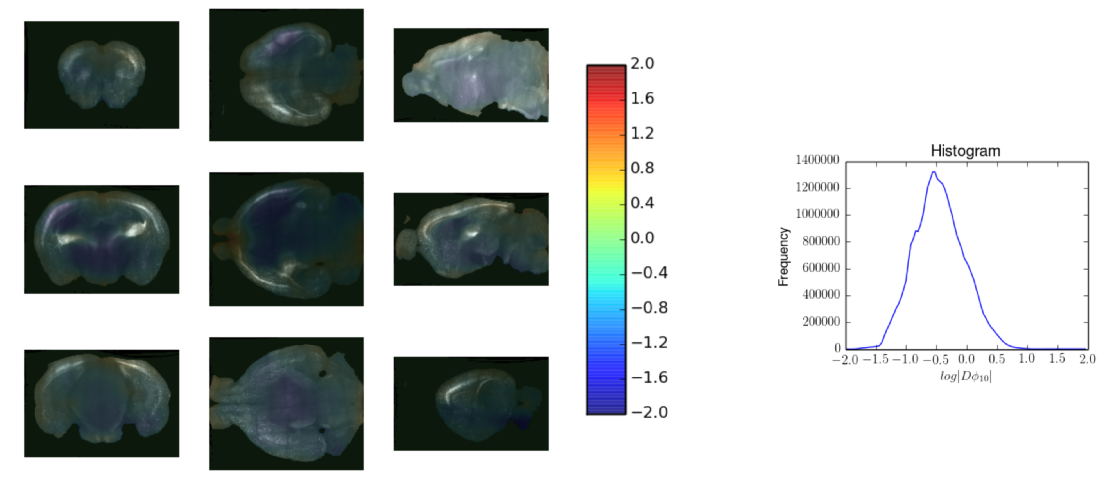
\includegraphics[width=.73\textwidth]{./figs/ndreg.png}
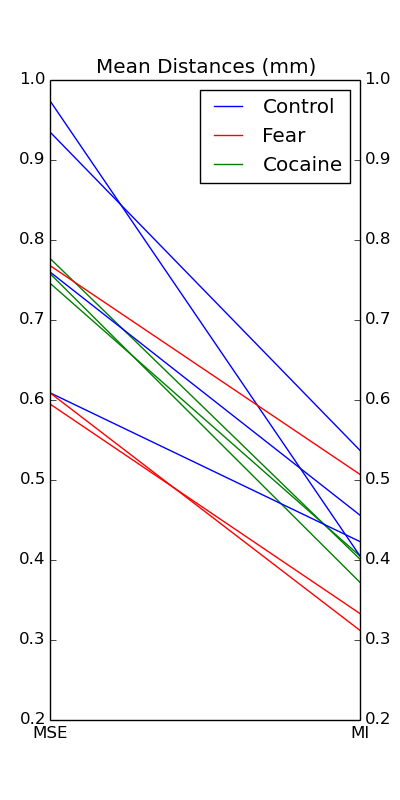
\includegraphics[width=0.25\textwidth]{./figs/ndreg-md.png}\\
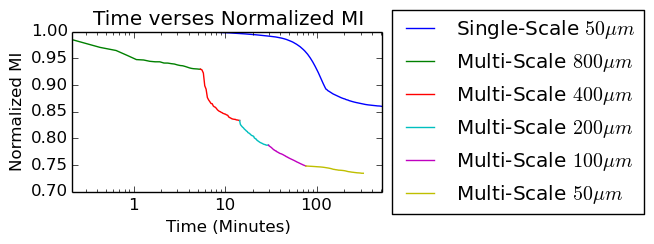
\includegraphics[width=0.75\textwidth]{./figs/ndreg-time.png}
\caption{
  The metric distance between the CLARITY and ARA was computed at the
  end point of the registration by integrating the time varying velocity
  fields from LDDMM.  It is a measure of how much the CLARITY brain
  differed from the ARA. The next figure compares the calculated
  distance when a Mean Square Error (MSE) cost is used during LDDMM to
  registration with Mutual Information (MI).  The metric distance was
  consistently smaller for MI under all 3 conditions (Control, Cocaine
  and Fear).  This indicates that the quality of the registration was
  higher than under a MSE cost.
}
\label{fig:ndreg}
\end{cframed}
\end{figure}

NeuroData’s registration module (ndreg) uses the Large Deformation
Diffeomorphic Metric Mapping (LDDMM) for image alignment.  LDDMM
computes a smooth invertible mapping between template image $I_0$ and
target image $I_1$. The plot below shows the timing results of experiments
registering a CLARITY brain template to the Allen Reference Atlas (ARA)
target.  In the first experiment the CLARITY image was registered to the
(ARA) using a single-scale approach on a 50 $\mu$~m grid.  In the second
experiment registration was done by a coarse to fine multi-scale method.
Registration that was done at a lower resolution was used to initialize
the algorithm at the subsequent higher resolution level.  Resolution
levels of 800, 400, 200, 100 and then 50 $\mu$~m were used. The Mutual
Information (MI) between the deformed CLARITY and ARA images was
normalized to a range of $[0, 1.0]$ where 1.0 indicates that no
registration occurred and 0 indicates the best possible scenario ($I_0 =
I_1$).  The plot in figure~\ref{fig:ndreg} shows that the multi-scale optimization was much faster
than the single-scale method.


\begin{figure}[h!]
\begin{cframed}
\centering
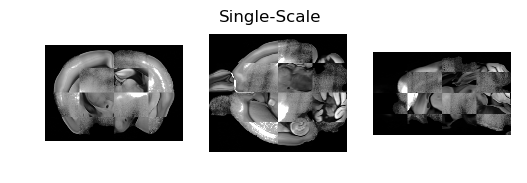
\includegraphics[width=0.75\textwidth]{./figs/ndreg-single.png}
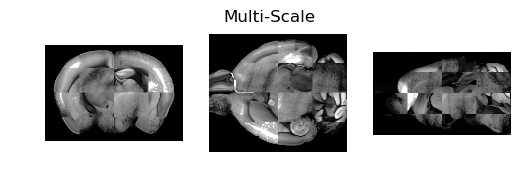
\includegraphics[width=0.75\textwidth]{./figs/ndreg-multiscale.png}
\caption{
  The images below are checkerboard composite images of the deformed
  CLARITY image and the ARA.  They show that usage of the multi-scale
  approach did not reduce registration quality when compared to the
  single-scale method.
}
\label{fig:ndregChecker}
\end{cframed}
\end{figure}

\end{document}
